\section{Optimizing the Basic Approach}
\label{sec:opt}

A large drawback of the MILP-based approach described in the previous section is
that it exhaustively encodes the combination of all tuples in the database and all queries
in the query log.  In this approach, the number of constraints grows quadratically with respect to
the database and the query log; the number of undetermined variables also increases quandratically.
Both of these properties typically .
In a simple experiment, shown in Figure~\ref{fig:querysize_vs_time}, we generated increasingly 
larger query logs for a database of $XXX$ tuples, encoded the problem using $\sys_{exh}$, and solved
the problem using an ILP-solver (CPLEX~\cite{cplex} in our experiments).
We find that the solver time increases exponentially as the number of encoded queries increases,
due exponential increase in the number of possible states for the undetermined variables.
Although the solver performance varies widely depending on the specific problem, this experiment 
illustrates the limitations of the naive approach.

\begin{figure}{h}
    \centering
        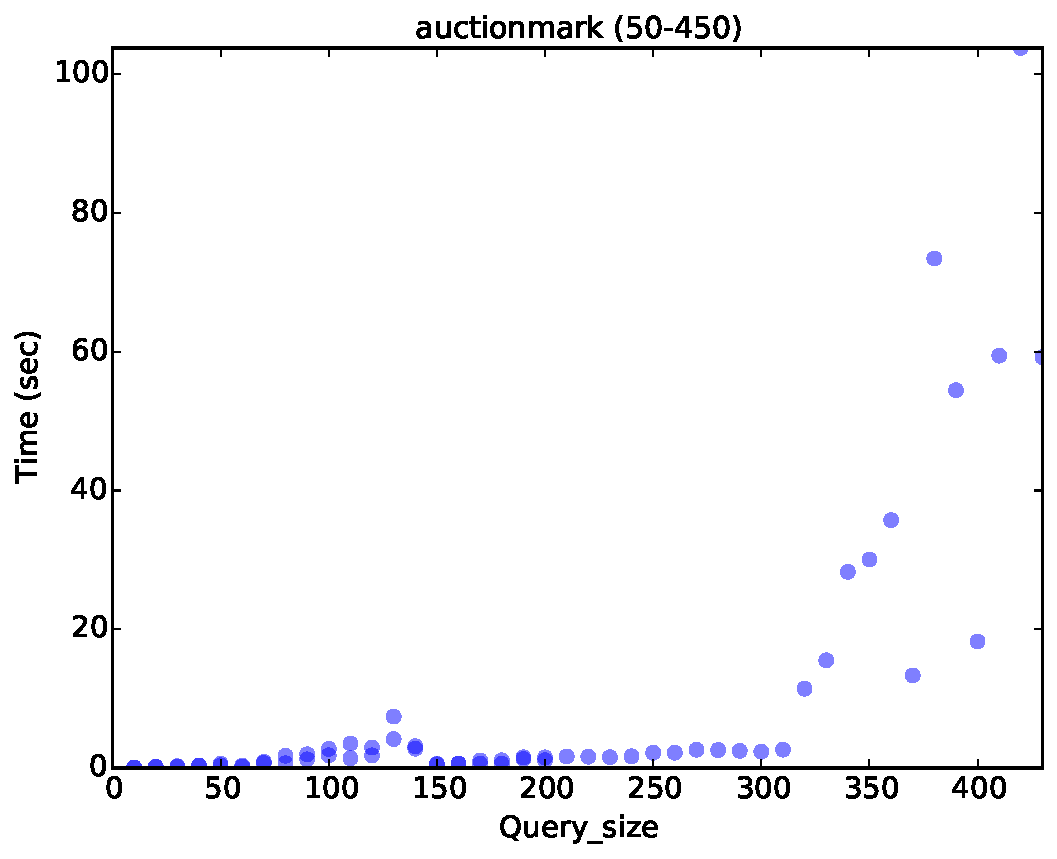
\includegraphics[width=0.4\textwidth]{figures/auctionmark_qsize_time}
    \caption{\# of queries vs. execution time on Auctionmark dataset. }
    \label{fig:querysize_vs_time}
\end{figure}

To resolve this limitation, we explored two classes of optimizations that seek to
reduce the number of encoded tuples and the number of linearized queries in the MILP problem.
In addition, incremental algorithm that is faster if the corruption is recent.  
We see in experiments that this is likely the case.




% In the previous section, we introduce the basic approach to derive
% the log repair by incorporating information from every query
% and every tuple into a single MILP problem. However, oftentimes, 
% this basic approach end up with 
% a huge problem as the query log size and table size increase. 
% In Figure~\ref{fig:querysize_vs_time}, 
% we observe that the total solver (IBM CPLEX) solving time 
% grows exponentially and 
% unpredictably as the query 
% log size or the table size increases. As a result, the basic approach does not scale over 
% large problems (large query log size and large table size).


linearize whole query log, so cost of adding an additional tuple is very high.
second iteration generally takes ~1 - 10%
for large databases knn cost is pretty high: ~

if the solver returns, it is always a super set of the clean range

only tuples modified by the fixed queries
- tuples already in the complaints (correct)
- not in complaints, but any of the originial queries modified it
- not in complaints, but no original queries modified it



\subsection{Reducing Tuples}
\label{sec:opt:tbsize}

We opt to aggressively reduce the number of tuples by only encoding the tuples
mentioned in the complaint set $\mathcal{C}$.
Derives an inaccurate log repair.  It is guaranteed by the problem formulation
that the fix will resolve the errors in $\mathcal{C}$.  However, because the problem
only encodes $\mathcal{C}$, there are certain problem settings where 
the resulting fix may not generalize to all of the tuples in the database, 
and thus introduce new errors.    
% However, there are cases
% where the predicate of the fixed query matches tuples were not part of $\mathcal{C}$.  
% In that case, it is possible that when the fixed query is applied to the database, 
% it will introduce new errors.

\begin{figure}[h]
    \centering
    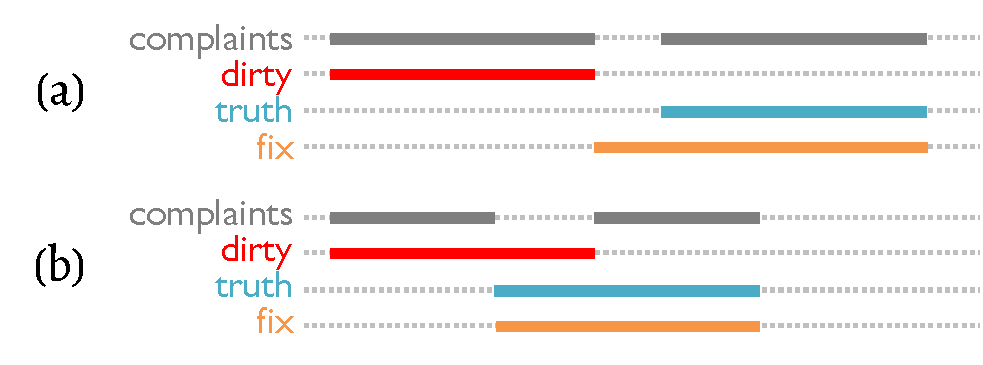
\includegraphics[width=0.4\textwidth]{figures/2nditerationgroups}
    \caption{Graphical depiction of the group 2 and group 3. }
    \label{fig:groups}
\end{figure}

Figure~\ref{fig:groups} depicts the two cases where the fixed query may contain tuples in the full
database that were not in $\mathcal{C}$.
Each solid and empty circle represents a tuple in the database that is in or not in $\mathcal{C}$, respectively.  
Each thick line represents the interval of query $q$'s single range predicate: 
dirty is the incorrect range in the corrupted version,
truth is the correct range in the true query, 
and fix is the range returned by the solver.
Recall that our goal is to reproduce the truth range given the tuples in $\mathcal{C}$ (solid circles)
and the dirty range.  

In (a), the dirty range overlaps with the true range, thus the tuples within the overlapping 
region are not complaints, are correctly modified by the dirty range, and should be included
in the fixed range.  In general, non-complaint tuples that match the fix query as well as 
the dirty range are by definition correctly part of the fixed range.

In contrast, consider (b), where the dirty and clean ranges are non-overlapping.
The non-complaint tuples shown should not be modified by $q$, and so the proposed
fix has incorrectly generalized.  In this case we use this additional information to
encode a second MILP problem to adjust the fixed range while taking the non-complaint tuples
into account.




% fix is always the smallest possible, so it can only require a sceond iteration if the dirty and clean
% ranges don't overlap at all.  
% 
% The basic solution, which suggests to linearize every tuple in the database into the MILP problem,
% has two major disadvantages: 1. the system may end up with a large MILP problem that requires 
% the solver to run forever to solve; 2. we can only linearize the every tuple
% when the complaint set is complete, which is often hard to guarantee. Thus, in the first 
% optimization, we propose a two-iteration approach handles both of these two problems 
% by linearizing tuples in the complaint set in
% the 1st iteration and refining the log repair in the 2nd iteration. \\
% \subsubsection{1st iteration}
% We use tuples in the complaints $\mathcal{C}$ to construct the MILP problem and derive a 
% inaccurate log repair $\mathcal{Q}^*$\xlw {we need to find a term for this}. This inaccurate 
% log repair resolves tuples in the complaints $\mathcal{C}$, but, at the same time, 
% introduces noises by over correcting tuples that are not involved in the MILP problem. 
% As shown in Example~\ref{ex:2nditer}, by resolving tuples in complaints $\mathcal{C}$, 
% the system derives a log repair that introduces other errors. 
% \begin{example}\label{ex:2nditer}
% Including tuples in the complaints $\mathcal{C}$ to solve problem in Example~\ref{ex:taxes2} 
% and using Euclidean distance of variables in the query as the objective function, the system 
% derives a log repair $\mathcal{Q}^*$ with $q_1^*=$ \texttt{\small UPDATE Taxes SET rate = 30}
% \texttt{\small WHERE income >= \color{red}{9500.0001} \color{black}{and income <=} \color{red}{90000}}. 
% This log repair resolve tuples in the complaints. However, the fixed query $q_1$ has a much wider range 
% and it it incorrectly modifies tuples that are not in the complaint, e.g., tuple $t_4$.
% \end{example}
% \ewu{why would this happen if we encoded all the tuples?  Doesn't the objective penalize this case?}
% 
% 
% To avoid introducing such noises, we introduce the 
% 2nd iteration which targets on refining the log repair derived in 
% the 1st iteration. 
% \subsubsection{2nd iteration}
% The goal for 2nd iteration is to optimize the impact of the log repair (tuples
% modified by $\mathcal{Q}$). 
% Let $\mathcal{Q}^*_{sub} = \mathcal{Q}^*-\mathcal{Q}$ as 
% queries modified in the log repair, in the 2nd iteration, we 
% construct a separate MILP problem by linearizing 
%  queries between the first and the last query in
% $\mathcal{Q}^*_{sub}$, parameterizing variables in 
% the where clause for queries in $\mathcal{Q}^*_{sub}$,
% and maximizing the log repair impact score. 
% 
% 
% We define the impact score by dividing the 
% impacted tuples $T$ into three groups and defining the 
% impact score accordingly. \xlw {we need to fix these terms}. 
% 
% \smallskip
% 
% \noindent\textbf{Group 1}: tuples in the complaints $\mathcal{C}$. Impact of 
% $\mathcal{Q}^*$ on this group
% are guaranteed as correct. \textbf{Rule:} 
% strictly satisfy, including these tuples as 
% constraints in the 2nd iteration MILP problem. 
% 
% \smallskip
% 
% \noindent\textbf{Group 2:} tuples not in $\mathcal{C}$, but also modified 
% by the original query log $\mathcal{Q}$. Impact of $\mathcal{Q}^*$ 
% on the group 2 are likely to
% be correct. \textbf{Rule:} adding these tuples into the 
% rewarded tuple set $T_{reward}$. 
% \ewu{what does "modified by the original query log Q mean?}
% 
% \smallskip
% 
% \noindent\textbf{Group 3:} tuples not in $\mathcal{C}$ and not modified 
% by the original query log $\mathcal{Q}$. Impact of 
% $\mathcal{Q}^*$ on the last group should penalized, thus 
% we put them into $T_{penalize}$ (\textbf{Rule}).
% 
% \smallskip
% 
% The impact score, which is also the objective function for
% the MILP problem, is $T_{reward} - T_{penalize}$. \ewu{what exactly is this objective function?  the number of tuples modified?}We further 
% optimize the 2nd iteration to reduce the size of $T$ 
% by searching for K-nearest-neighbors
% of tuples in complaints $\mathcal{C}$. 
% There are multiple benefits for the two-iteration approach:
% \begin{itemize}
% \item It minimizes the size of MILP problem in the 1st iteration. 
% \item It refines the log repair while avoid over correcting tuples not in 
% the complaints $\mathcal{C}$. 
% \item It pptimizes the impacted tuples efficiently by controlling the queries 
% and number of impacted tuples
% involved in the 2nd MILP problem.
% \item In addition, it handles cases when we don't have complete complaints
% $\mathcal{C}$ (false negatives). 
% \end{itemize}



\subsection{Optimization: log size}


\if{0}
\subsubsection{A Naive but Flawed approach}
\ewu{Better explained as: CPLEX searches through an exponential space of all possible combinations of MILP variables.  In a chunked approach, the solution of each chunk is one out of a potentially arbitrary number of possible solutions, thus it is easy to pick an incorrect one}
A natural idea to optimize the basic approach is 
to \textbf{chunk the query log} into
smaller, fixed size pieces and then solve each piece at a time: starting
from the most recent piece, the system linearizes and parameterizes queries 
in the current piece and derives a corresponding log repair; 
it then examines the other pieces iteratively
in the same way. Since complaints only provides
true values for the most recent database state, in order to avoid 
linearizing additional queries, 
we need to know \textbf{rollback} the true values of tuples 
until the last query in each query log piece. \\
However, rollback the database is non-easy. An ideal, precise rollback
algorithm would generate a set of valid ranges for each attribute of a tuple. 
But the size of valid ranges also grows exponentially with the number queries
we want to rollback, which, in turn, could not improve the system performance. 
On the other hand, an approximate, imprecise 
rollback algorithm would either make the rest of the problems
infeasible to solve (only maintain fixed number of valid ranges) 
or result in deriving 
incorrect log repairs (maintain the lower 
bound and upper bound among all valid ranges).
  

In order to improve the system performance without losing accuracy, we propose
the following two optimizations: query-slicing optimization 
based on provenance over queries and
attribute-slicing optimization based on provenance over 
attributes. 
\fi

\subsubsection{Query-Slicing}
\label{sec:opt:query}
The exhaustive parameterization of all queries in the query log, as described
in the basic approach, is typically unnecessary because many queries in the log
could not have affected the tuple attribute values in the complaint set.
To avoid such redundant computation, \textit{query-slicing} 
removes \texttt{UPDATE} queries whose \texttt{SET} clauses did not modify 
attributes that could possibly have affected the {\it complaint attributes} 
specified in the complaint set.

\ewu{changed INcorrect attributes to Complaint Attributes}

\begin{definition} [Complaint Attributes]
	The complaint attributes $\mathcal{A}(C)$ are attributes in 
	table $R$ with incorrect values: 
	\[\mathcal{A}(C) = \{A_i|A_i\in R, \exists t.A_i \neq t.A_i^*, t\in C\}\]
\end{definition} 

\ewu{Why don't we use lineage/provenance language?}
\begin{definition}[Query dependency\& impact]
    The \textbf{dependency}, $\mathcal{P}(q)$, of a query $q$
    is the set of 
    attributes involved in the condition function of $q$:
    \[\mathcal{P}(q) = \Pi_{f_{q}.\sigma}(R)\]
    The \textbf{direct-impact} of query $q$, denoted
    by $\mathcal{I}(q)$, is the set of attributes 
    involved in the update function of $q$:
    \[\mathcal{I}(q) = \Pi_{f_{q}.\mu}(R)\]
    The \textbf{full-impact}
    of $q$, $\mathcal{F}(q)$, propogates the $q$'s direct impact through
    the subsequent queries in the query log to describe {\it all} attributes
    that are affected by the changes caused by $q$'s \texttt{SET} clause.
    We describe its implications and calculation next.
    \ewu{Is this correct?}
\end{definition}


By comparing $\mathcal{F}(q)$ and $\mathcal{A}(C)$, we know whether
or not corrupting query $q$'s parameters could possibly have caused the complaint
set.  Specifically, when $|\mathcal{F}(q) \cap \mathcal{A}(C)|=|\mathcal{A}(C)|$, 
$q$ potentially affected all of the attributes referenced in the complaint set and is
a candidate for fixing; 
when $0 < |\mathcal{F}(q) \cap \mathcal{A}(C)|< |\mathcal{A}(C)|$, 
$q$ contributed to a subset of the attributes in the complaint set; 
and when $|\mathcal{F}(q) \cap \mathcal{A}(C)|=0$, $q$ is irrelevant 
and can be ignored as a candidate for fixing. 
We use $Rel\mathcal{(Q)}$ to denote the set of relevant queries. 

Algorithm~\ref{alg:fullimpact} describes how we find
$\mathcal{F}(q_i)$ for $q_i$ in the query log:

\begin{algorithm}[htbp]
\caption{$FullImpact$ algorithm for finding $\mathcal{F}(q)$.}
\label{alg:fullimpact}
\begin{algorithmic}
\REQUIRE {$\mathcal{Q}$, $q_i$}
% \ENSURE {$\mathcal{F}(\mathcal{Q})=\{\{\mathcal{F}(q_1)\}, ..., \{\mathcal{F}(q_n)\}\}$}
% \FOR {each $q_i$ in $q_n, ..., q_1$}
\STATE $\mathcal{F}(q_i) \leftarrow \mathcal{I}(q_i)$
\FOR {each $q_j$ in $q_{i+1}, ..., q_{n}$}
\IF {\red{$\mathcal{F}(q_i)\cap \mathcal{P}(q_j) \neq \emptyset$}}
\STATE $\mathcal{F}(q_i) \leftarrow \mathcal{F}(q_i) \cup \mathcal{F}(q_j)$
\ENDIF
\ENDFOR
\STATE $\mathcal{F}(\mathcal{Q}) \leftarrow \mathcal{F}(\mathcal{Q}) \cup {\red{\{\mathcal{F}(q_i)\}}}$
% \ENDFOR
\STATE Return $\mathcal{F}(\mathcal{Q})$
\end{algorithmic}
\end{algorithm}

Finally, we can compute $Rel\mathcal{(Q)}$



\subsubsection{I don't understand this}


In addition to pruning out irrelevant queries,
we also prune irrelevant attributes. \\
Let $Rel\mathcal{(Q)}$ as the set of 
relevant queries, we can find the relevant 
attributes as following:
\[Rel\mathcal{(A)} = \cup_{q_i \in Rel\mathcal{Q)}} 
(\mathcal{F}(q_i)\cup \mathcal{P}(q_i)) \]



\subsubsection{Incremental Computation}

\begin{figure}[t]
  \centering
  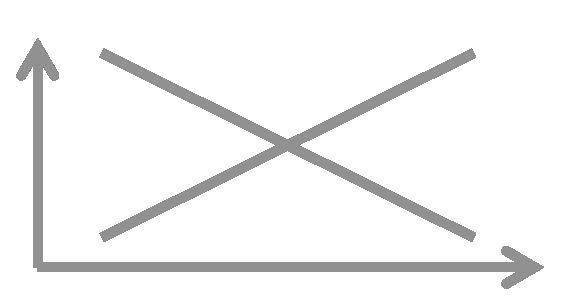
\includegraphics[width=.4\textwidth]{figures/placeholder}
  \caption{Solver time vs size of encoded query log.}
  \label{fig:badscaling}
\end{figure}

\ewu{Need to justify why we incremental algorithm steps back query at a time given Figure~\ref{fig:querysize_vs_time} suggests parameterizing >1 query is the same speed.}

Despite the previous optimizations, it is still expensive to parameterize all 
queries in $Rel\mathcal{(Q)}$ and solve for all parameterized values.
In particular, the cost of solving a MILP problem increases \ewu{cubically?}
with respect to the number of variables.
For example, Figure~\ref{f:badscaling} shows the time cost of the CPLEX solver
as we increase the number of query logs that are encoded and sent to the solver.  
The solid line is when the values in all of the queries are parameterized, while
the dashed line illustrates the time if only the oldest query is parameterized. 
These results suggest that it is {\it faster} to run a separate MILP problem for each 
suffix of the query log (e.g., $q_i, \ldots, q_m$) where $q_i$ is parameterized, 
rather than encode and parameterize the entire log.
Thus we use use an incremental approach, where we individually test each relevant query from the most recent
to the oldest:


\begin{algorithm}[htbp]
\caption{$QueryFix_{inc}$ algorithm.}
\label{alg:incalg}
\begin{algorithmic}
\REQUIRE {$Rel\mathcal{(Q)}$}
\STATE Sort $Rel\mathcal{(Q)}$ from most to least recent
\FOR {each $q_i \in Rel\mathcal{(Q)}$}
  \STATE $q_i^*$ $\leftarrow$ $QueryFix(\{q_j | j \ge i \wedge q_j \in Rel\mathcal{(Q)}\})$
  \IF {$q_i^* \neq \emptyset$}
    \STATE Return $q_i^*$
  \ENDIF
\ENDFOR
\end{algorithmic}
\end{algorithm}



A benefit of this approach is that complaints are more likely to be the result of
recent queries rather than very old queries, and our experiments in Section~\ref{exp:}
speak towards this point.




